% !TEX root = ../main.tex

\chapter{Literature review}
\label{ch:literature_review}
%Traditionally, building a CAD system consisted of two different steps: "Lesion  detection (CADe) and  false-positive  reduction (CADx).  Lesion  detection  was  primarily  based  on  algorithms  specific  to  the  detection task, resulting in many candidate lesions. False-positive reduction was commonly based on traditional  machine  learning  methods  to  reduce  the  false  positive  rate. However,  even  with  these  complicated and sophisticated programs, the general performance of conventional CAD systems was not good, thus hampering their widespread usage in clinical practice"~\cite{41}.\\
%Nowadays, these two steps tend to disappear thanks to deep learning algorithms, in particular the ones based on convolutional neural networks. In fact, the latter can be considered as single-step CAD system. For this reason, CAD systems are currently a trending topic in deep learning.\\

\setlength{\marginparwidth}{3cm}\leavevmode \marginnote{\textbf{Johan}}Since this work focuses on lesion classification, this chapter presents the main research works about CAD systems based on convolutional neural networks for each body part used in sections \ref{ch:paper_reproduction} and \ref{ch:transfer_learning}, i.e. prostate, lung and brain. Furthermore, it exclusively focuses on studies that used the same datasets as the ones used in this work.

\section{Prostate/PROSTATEx}

\setlength{\marginparwidth}{3cm}\leavevmode \marginnote{\textbf{Julien}}As stated by Gao et al., "Prostate  cancer  is  the  most  common  malignancies  among  men  and  remains  a  second  leading  cause to deaths in men globally. It was predicted that there would be 1.7 million new cancer cases by 2030. The early detection and diagnosis of prostate cancer can help to survive nine out of 10 men for the last five years"\cite{41}. Therefore, researchers proposed many different models to achieve good performance in prostate cancer detection. All the research works mentioned below are based on the SPIE-AAPM-NCI PROSTATEx Challenge dataset. This dataset is composed of multiparametric MRIs (T2W, DWI, ADC, DCE, PD, Ktrans) for a total of 204 training patients and 208 challenge patients (see Section \ref{sec:prostatex_dataset_description}).\\ \\
Song et al.~\cite{07} presented a DCNN method to detect prostate cancer on multiparametric MRIs. Their data processing approach kept T2W, DWI and ADC grayscale images only. After resampling each image to the same resolution, T2W, DWI and ADC images were first cropped ($65$x$65$px patch) with the lesion in the center and stacked per patient, resulting in images containing three grayscale channels. Thanks to this method, the same lesion is visible in the same area over the three channels. This increases the probability of detecting a cancer by ensuring a good visibilty for each lesion, since the latter is not necesarily as visible with each parameter. Images were then normalized based on the Z-score per patient and per sequence (T2W, DWI, ADC), i.e. by subtracting the mean before dividing by the standard deviation. The data was split into a training ($80\%$), validation ($10\%$) and test set ($10\%$). The training (undefined number of times), validation (undefined number of times) and test images (11x) were augmented using -20$^\circ$ to 20$^\circ$ rotations, horizontal flipping, vertical sliding of less than 2 pixels and stretching by a factor between 0.9 and 1.1. Most of the processing techniques are reproductible, apart from the manual lesion contouring and labelling performed by a radiologist. 
Their model is a modified version of the well-known VGG16 model, including the addition of $1$x$1$ convolutions and dropout layers after each max pooling layer, and the use of the ELU activation function (see figure \ref{fig:paper_model}). The evaluation method for each patient and finding made an average of the 11 predictions resulting from the 11-time augmentation of the test set. The best results were obtained by using DWI images only with the highest b-value, reaching an AUC of $0.944$ with a 95$\%$ confidence interval ($0.876$-$0.994$). However, this model was not tested on the official PROSTATEx challenge images, which is an interesting benchmark to evaluate how well a model generalizes.\\ \\
Liu et al.~\cite{46} created another architecture called XMasNet which was tested on the actual PROSTATEx challenge, achieving the second best performance at the time with an AUC of $0.84$. The AUC on their validation set reached $0.92$. Regarding data processing, their approach stacked different combinations of the available sequences as the three channels instead of defining a single combination like Song et al.: DWI-ADC-Ktrans, DWI-ADC-T2W, ADC-Ktrans-T2W and DWI-Ktrans-T2W. The data augmentation process differs in that the images are rotated in 3D, each lesion being sliced at 7 different orientations. These 2-dimensional slices were then augmented using rotation, shearing and translation of 1px, resulting in 207144 training samples. Both validation and testing test were also augmented in the same manner. This whole process allows to include 3-dimensional information in 2-dimensional images. The method used ensemble learning which combined different models to reach the best performance possible.\\ \\
Mehrtash et al.~\cite{01} used a different approach. First of all, the input was fed to three separated parts of the model, each one responsible for a specific sequence among ADC, maximum b-value DWI and Ktrans. Then, each of these feature extractors' outputs were merged into a common decision maker. Furthermore, 3-dimensional convolutions instead of 2-dimensional ones were performed. In fact, 3-dimensional patches centered on the lesion were cropped. Augmentation including translation and flipping was used in order to balance the dataset. Apart from these differences, other minor differences such as normalizing the images within the range $[0,1]$ exist compared to the previous papers. These tricks allowed their model to achieve an AUC of $0.80$ on the PROSTATEx challenge. To make predictions, five different models were used, averaging the predictions of the four best models.\\ \\
Armato et al~\cite{42} summarized the results obtained by all teams that took part in the PROSTATEx challenge in 2017. This challenge was split into two separate tasks. The first one was devoted to the diagnosis of prostate lesions (classification) whereas the other was about the segmentation and the determination of Gleason Grade Group. Thirty-two groups submitted results to the first challenge out of a total of 71 different methods (each group was allowed to submit up to three methods for evaluation). The article indicates that "most, but not all, methods outperformed random guessing (AUC=0.5)"~\cite{41}. The best performing method obtained an AUC value of 0.87 (standard error 0.027) and the next three methods all achieved AUC values of 0.84 (with standard errors of 0.036, 0.032, and 0.032). The complete results are illustrated on figure \ref{fig:challenge_all_results}. The median AUC on the challenge is approximately $0.68$.
\begin{figure}[!h]
\centering
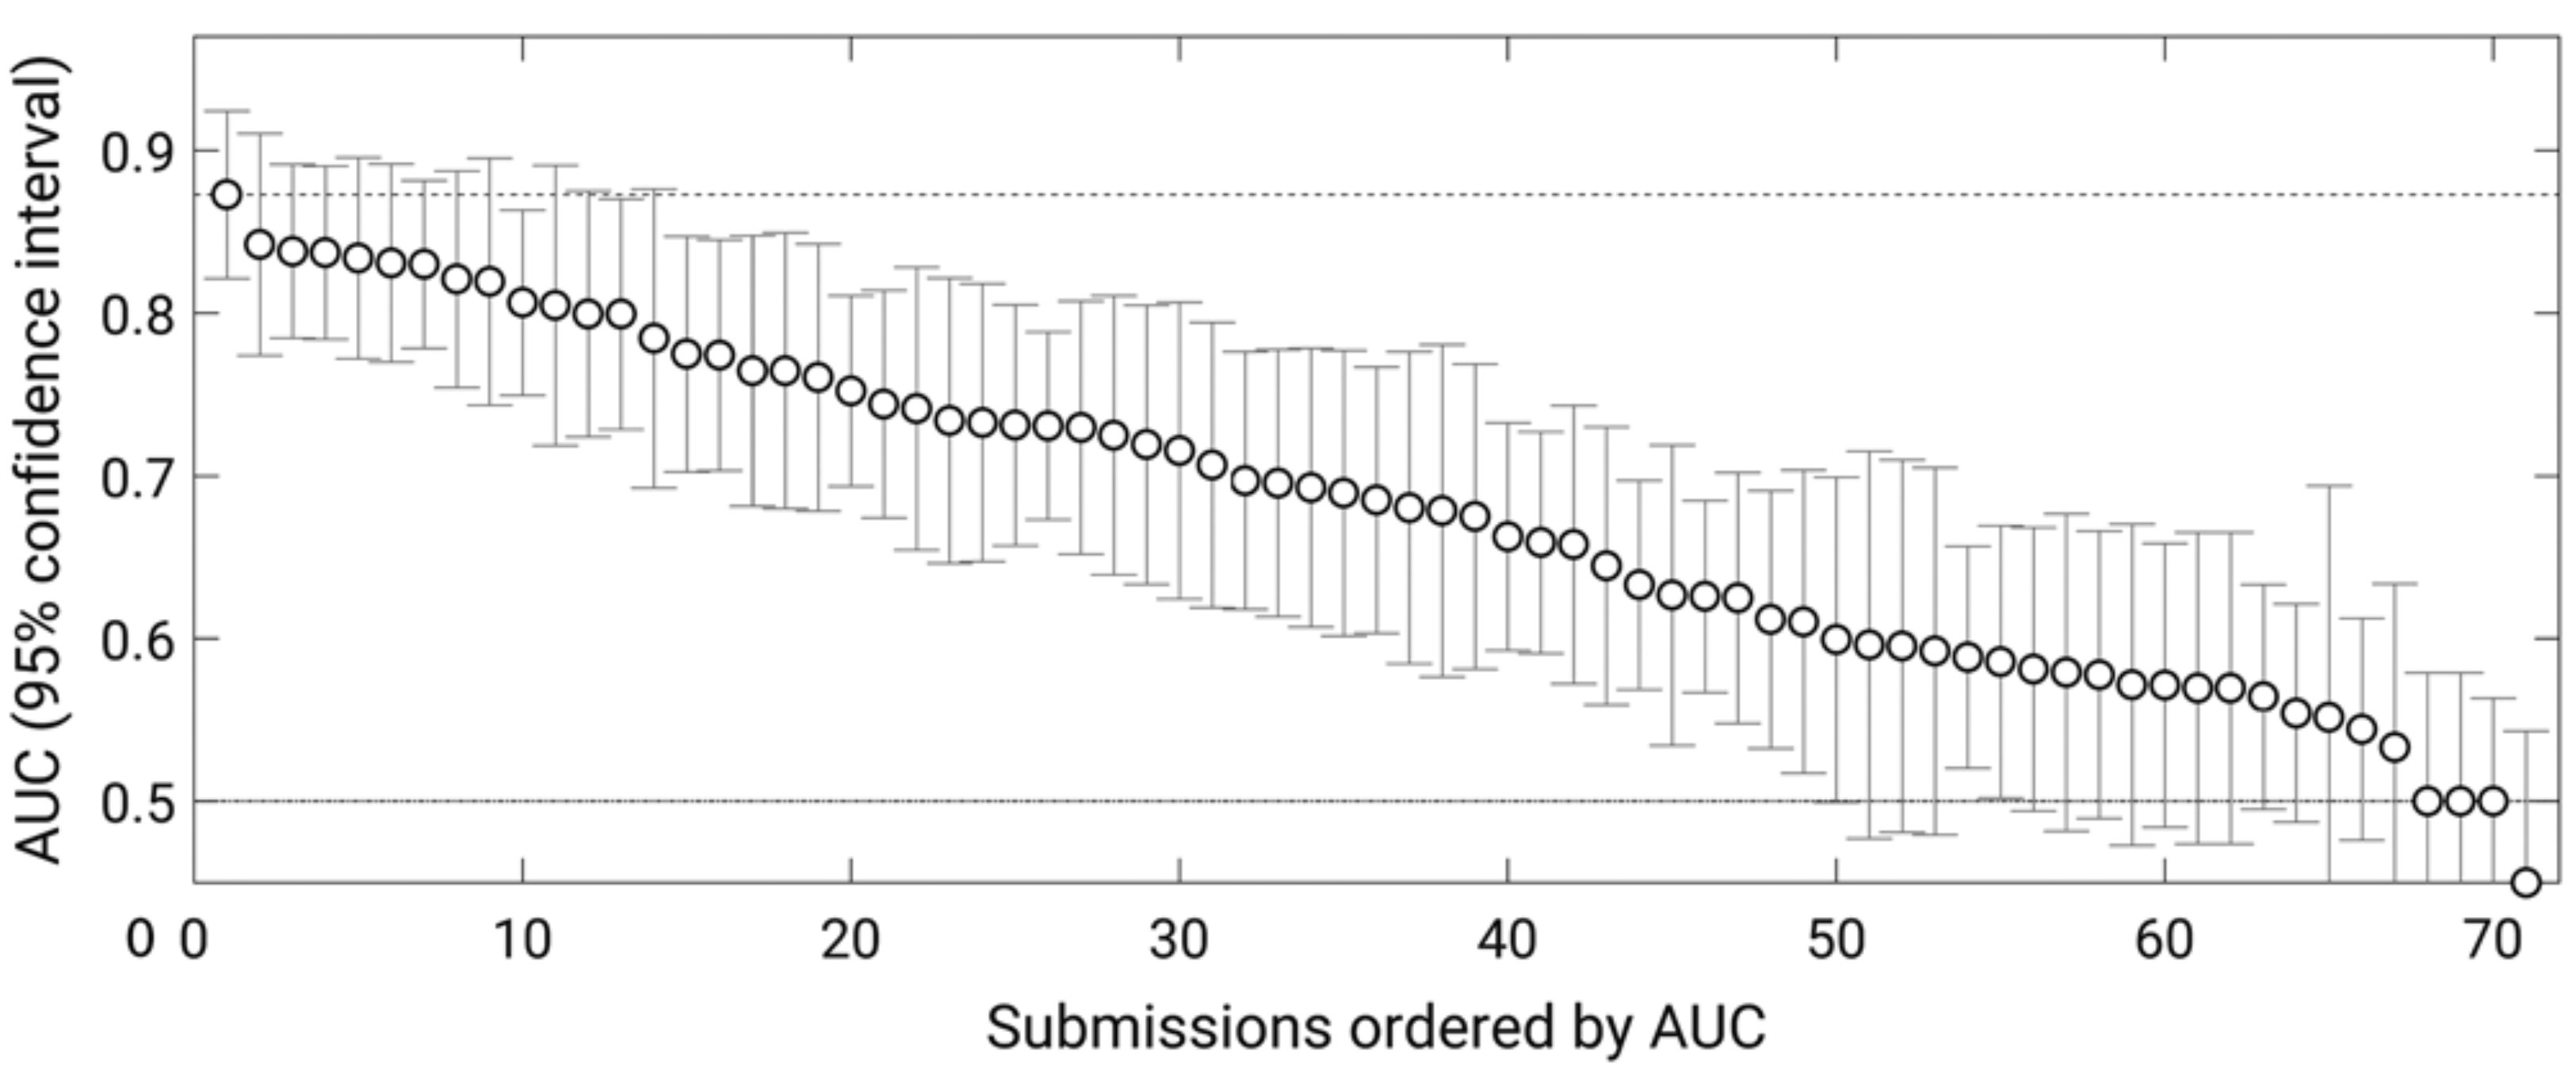
\includegraphics[width=1\textwidth, keepaspectratio=true]{./figures/challenge_all_results.png}
\caption{AUC values achieved by the 71 methods that participated in the PROSTATEx Challenge~\cite{42}}
\label{fig:challenge_all_results}
\end{figure}


\section{Lung/Lung CT Challenge}
\setlength{\marginparwidth}{3cm}\leavevmode \marginnote{\textbf{Johan \& Julien}}Gao et al. claimed that "lung cancer is one of the most frequent and leading causes of death all over the world. It was reported that there were approximately $1.8$x$10^6$ new cases of lung cancer globally in 2012. Early detection of lung cancer, which is typically viewed in the form of lung nodules, is an efficient way to improve the survival rate"~\cite{41}. The articles cited below make use of the SPIE-AAPM Lung CT Challenge dataset, which is composed of CT scans devoted to the classification of lung nodules (see \ref{sec:lungCTChallenge} for further details).\\ \\
Cengil et al.~\cite{02} built a fairly simple convolutional neural network to classify the images of the Lung CT Challenge dataset. The model takes 4-dimensional data as input (depth, height, width and channels) and performs 3D convolutions on it. The model consists of an input layer, five layers of 3D convolutions (the first is associated with a RELU activation function and pooling, the last with nothing, and the others with pooling) and a fully connected layer at the end. Regarding the model evaluation, authors announce an accuracy of 0.7 on their test set which contains 30 findings.\\ \\
Armato et al.~\cite{12} described the LUNGx Challenge and the overall results. This challenge consisted in classifying the lung nodules as benign or malignant among a training set of 10 scans and a test set of 60 scans. Since the training set was extremely small, training the model on other datasets was allowed. The article describes the results of the proposed methods and compares them with the performance of six qualified radiologists on the same task. The article reports that "ten groups applied their own methods to 73 lung nodules (37 benign and 36 malignant) that were selected to achieve approximate size matching between the two cohorts. Area under the receiver operating characteristic curve (AUC) values for these methods ranged from 0.50 to 0.68. Only three methods performed statistically better than random guessing. The radiologists’ AUC values ranged from 0.70 to 0.85. Three radiologists performed statistically better than the best-performing computer method."~\cite{12}. Figure \ref{fig:LUNGx_challenge_all_results} gives an overview of the results.

\begin{figure}[!h]
\centering
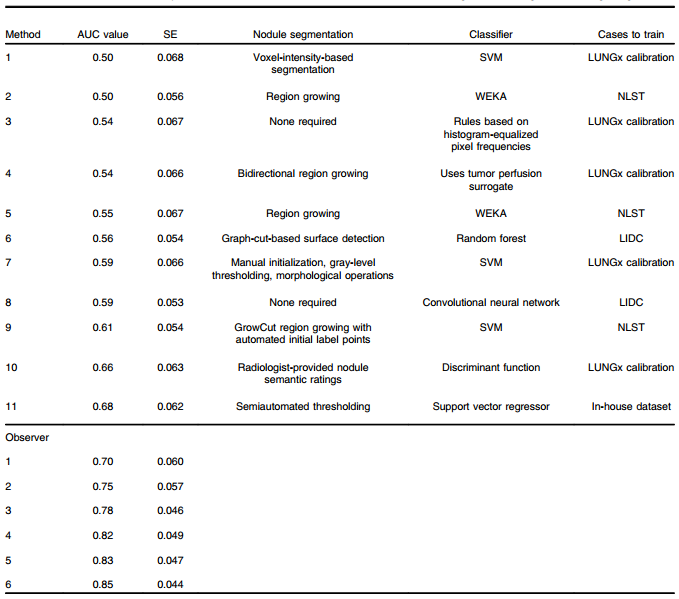
\includegraphics[width=1\textwidth, keepaspectratio=true]{./figures/LUNGx_challenge_all_results.png}
\caption{AUC values for the 11 computerized methods and six radiologists in the task of classifying malignant and benign nodules~\cite{12}}
\label{fig:LUNGx_challenge_all_results}
\end{figure}



\section{Brain/Kaggle Brain}

\setlength{\marginparwidth}{3cm}\leavevmode \marginnote{\textbf{Johan}}Brain cancer is another major type of cancer. According to American Society of Clinical Oncology, "brain and other nervous system cancer is the 10th leading cause of death for men and women. It is estimated that 17760 adults (9910 men and 7850 women) will die from primary cancerous brain and central nervous system tumors this year"~\cite{43}. The following research papers are based on the Kaggle "Brain MRI Images for Brain Tumor Detection" dataset. This dataset, unlike the ones for the other body parts, does not come from a certified medical authority but from the Kaggle website \cite{45}. However, as it is the only dataset available for brain tumor classification, some publications used it. Further details can be found in section \ref{sec:kaggleBrain}.\\ \\
Saxena et al.~\cite{31} implemented three convolution neural networks to classify the brain tumors coming from the Kaggle "Brain MRI Images for Brain Tumor Detection" dataset. Their processing method used a cropping technique which removed extra black margin around the skull. Each border of the image merged with a part of the skull. Since the images come from different sources, their resolution vary quite a lot. Therefore, the authors resized them to $224$x$224$x$3$. Moreover, data was augmented by rotation, vertical shifting and horizontal shifting. As the cropping was performed before augmenting the images, small parts of the brain were outside of the augmented images due to rotation and shifting. The data was split into a training set, a validation set and a test set. Regarding the models, authors implemented three of them (a Resnet-50, a VGG-16 and an Inception-V3) in order to compare their performance. The best results on the test set were achieved by the Resnet-50 (AUC of $0.95$ and accuracy of $0.95$). The VGG-16 was close (AUC of $0.90$ and accuracy of $0.90$), whereas the Inception-V3 didn't perform well (AUC of $0.55$ and accuracy of $0.55$).\\ \\
%Hanwat et al.~\cite{32} implemented a convolutional neural network to classify brain tumors of the Kaggle dataset. Their processing method included skull masking, i.e. the removal of every non-brain tissue from the image. According to the authors, this technique improves performance quite a lot. ---> Check their methods (graphs look special)
Habib Mohamed Ali~\cite{04} proposed his own convolutional neural network to classify the images of the Kaggle Brain dataset. First, the data was augmented. Then, it was cropped thanks to OpenCV so that the resulting images only contained the brain itself. Afterwards, they were resized and normalized in order to scale pixel values to the range $[0,1]$. Once the processing part was over, the data was split into a training set ($70\%$), a validation set ($15\%$) and a test set ($15\%$). Regarding the neural network structure, the model is simple. It is composed of only one convolutional layer with a batch normalization layer and ReLU activation function, followed by two max-pooling layers and a dense layer. This model achieved an accuracy of $89\%$ on the test set.

